% begin module eliminate-parameter-ex
\begin{frame}
\begin{example}
Sketch and identify the curve defined by the parametric equations
\abovedisplayskip=2pt
\belowdisplayskip=2pt
\[
\alert<handout:0| 15>{x = -t^2 + 2}, \qquad \alert<handout:0| 14>{y = t - 1}.
\]
\begin{columns}[c]
\column{.55\textwidth}
\ \only<handout:0| -2>{%
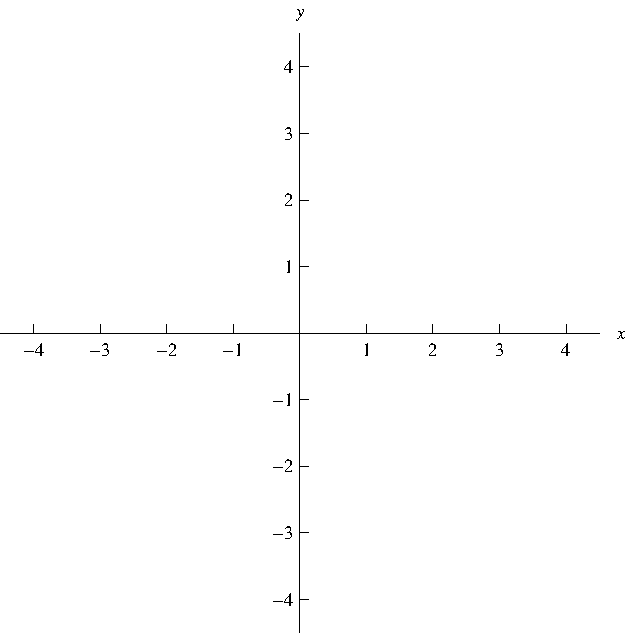
\includegraphics[height=6cm]{parametric-curves/pictures/11-01-ex1a.pdf}%
}%
\only<handout:0| 3-4>{%
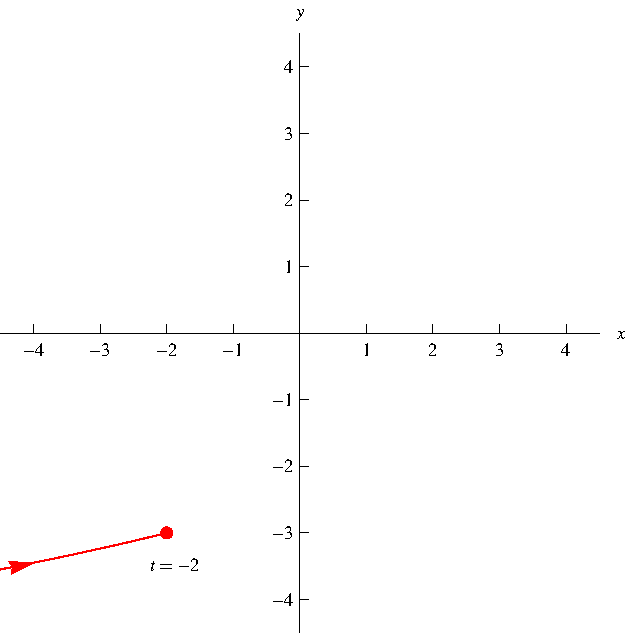
\includegraphics[height=6cm]{parametric-curves/pictures/11-01-ex1b.pdf}%
}%
\only<handout:0| 5-6>{%
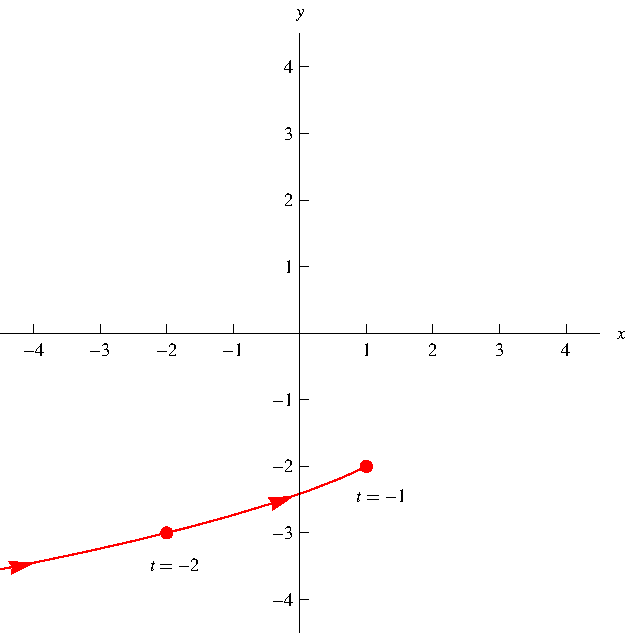
\includegraphics[height=6cm]{parametric-curves/pictures/11-01-ex1c.pdf}%
}%
\only<handout:0| 7-8>{%
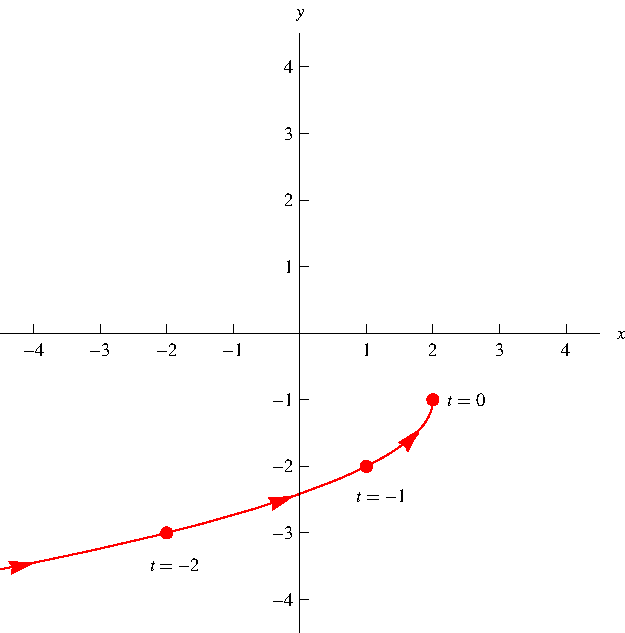
\includegraphics[height=6cm]{parametric-curves/pictures/11-01-ex1d.pdf}%
}%
\only<handout:0| 9-10>{%
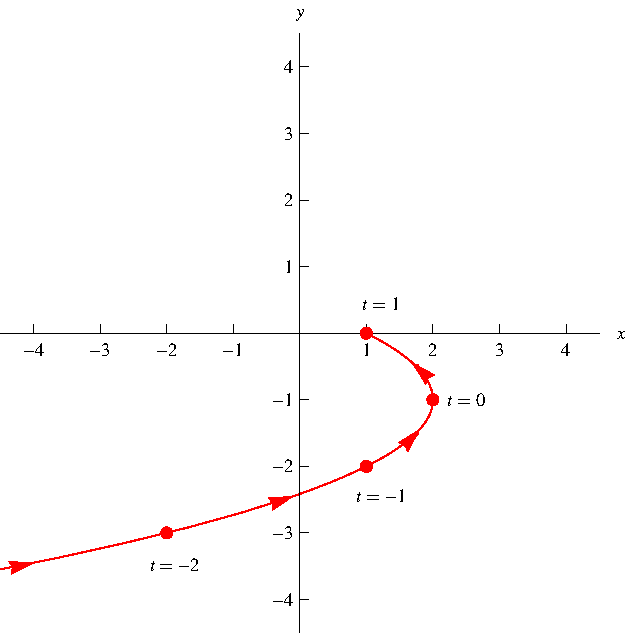
\includegraphics[height=6cm]{parametric-curves/pictures/11-01-ex1e.pdf}%
}%
\only<handout:0| 11>{%
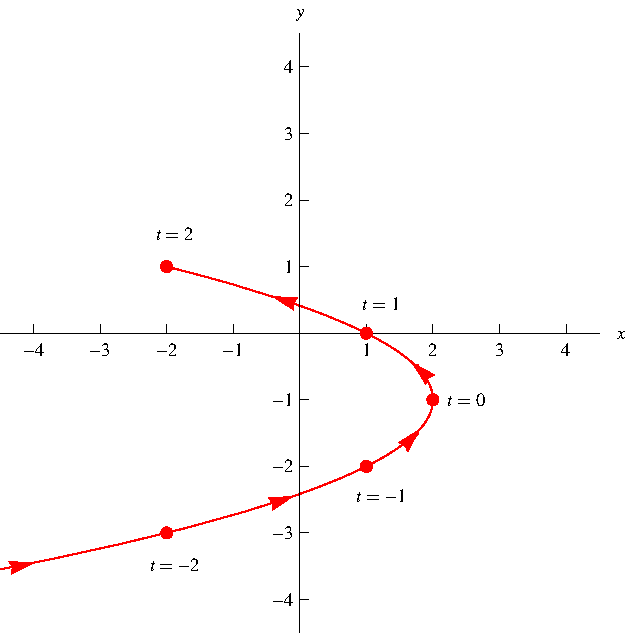
\includegraphics[height=6cm]{parametric-curves/pictures/11-01-ex1f.pdf}%
}%
\only<12->{%
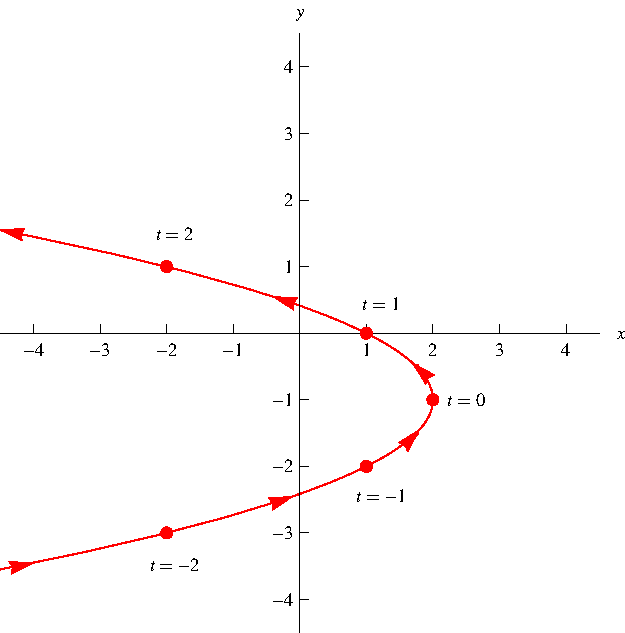
\includegraphics[height=6cm]{parametric-curves/pictures/11-01-ex1g.pdf}%
}%
\column{.45\textwidth}
\[
\begin{array}{|r|r|r|}
\hline
t & x & y\\
\hline
\alert<handout:0| 2-3>{-2} &%
\alert<handout:0| 2-3>{\uncover<3->{-2}} &%
\alert<handout:0| 2-3>{\uncover<3->{-3}} \\%
\alert<handout:0| 4-5>{-1} &%
\alert<handout:0| 4-5>{\uncover<5->{1}} &%
\alert<handout:0| 4-5>{\uncover<5->{-2}} \\%
\alert<handout:0| 6-7>{0} &%
\alert<handout:0| 6-7>{\uncover<7->{2}} &%
\alert<handout:0| 6-7>{\uncover<7->{-1}} \\%
\alert<handout:0| 8-9>{1} &%
\alert<handout:0| 8-9>{\uncover<9->{1}} &%
\alert<handout:0| 8-9>{\uncover<9->{0}} \\%
\alert<handout:0| 10-11>{2} &%
\alert<handout:0| 10-11>{\uncover<11->{-2}} &%
\alert<handout:0| 10-11>{\uncover<11->{1}} \\%
\hline
\end{array}
\]
\uncover<14->{%
Eliminate the parameter $t$: We get $\alert<handout:0| 14,16>{t = y + 1}$ from the second equation.  %
}%
\uncover<15->{%
Then%
}%
\abovedisplayskip=2pt
\belowdisplayskip=2pt
\begin{eqnarray*}
\uncover<15->{%
\alert<handout:0| 15>{x}%
}%
&\uncover<15->{\alert<handout:0| 15>{ =}}&%
\uncover<15->{%
\alert<handout:0| 15>{ -\alert<handout:0| 16>{t}^2 + 2}%
}\\%
& \uncover<16->{ = }&%
\uncover<16->{%
 -(\alert<handout:0| 16>{y+1})^2 + 2
}\\%
& \uncover<17->{ = }&%
\uncover<17->{%
-y^2 - 2y + 1
}%
\end{eqnarray*}
\end{columns}
\end{example}
\end{frame}

\begin{frame}
\begin{columns}[c]
\column{.5\textwidth}
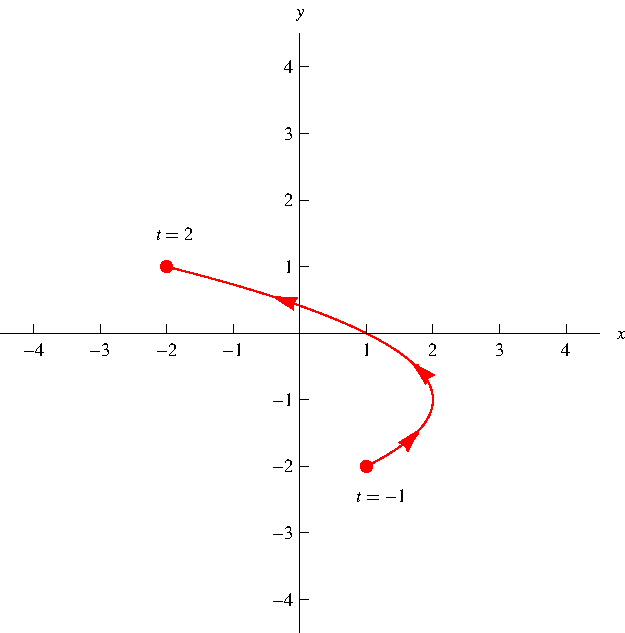
\includegraphics[height=6cm]{parametric-curves/pictures/11-01-ex1chopped.pdf}%
\[
x = -t^2 + 2, \qquad y = t - 1,
\]
\[
 -1 \leq t \leq 2
\]
\column{.5\textwidth}
\begin{itemize}
\item  There was no restriction placed on $t$ in the last example, so we assumed $t$ could be any real number.
\item  Sometimes we restrict $t$ to lie in a finite interval.
\item  For example, the parametric curve on the left is the part of the parabola from the previous example that begins at $(1,-2)$ and ends at $(-2,1)$.
\item  Here $(1,-2)$ is called the initial point and $(-2,1)$ is the terminal point.
\end{itemize}
\end{columns}
\end{frame}
% end module eliminate-parameter-ex
